%%%%%%%%%%%%%%%%%%%%%%%%%%%%%%%%%%%%%%%%%%%%%%
%                insertmeeting
% 1) Title (something creative & funny?)
% 2) Date (MM/DD/YYYY)
% 3) Location (ex. Hagerty High School)
% 4) People/Committees Present 
% 5) Picture 
% 6) Start Time & Stop Time (ex. 12:30AM to 4:30PM)
%%%%%%%%%%%%%%%%%%%%%%%%%%%%%%%%%%%%%%%%%%%%%%
\insertmeeting 
	{Organizing Outreach} 
	{08/18/21}
	{Hagerty High School}
	{Annika, Falon, Jensen, Nathan, Ritam, Rose, Samantha}
	{Images/RobotPics/robot.jpg}
	{1:30 - 4:30}
	
\hhscommittee{Outreach}
\noindent\hfil\rule{\textwidth}{.4pt}\hfil
\subsubsection*{Goals}
\begin{itemize}
    \item Discuss future plans for Outreach and come up with more challenging/unique outreach opportunities for our team.  

\end{itemize} 

\noindent\hfil\rule{\textwidth}{.4pt}\hfil

\subsubsection*{Accomplishments}
We started off by throwing random ideas back and forth, while refreshing our memories on which events have worked well for us in the past. Someone suggested that we could do teaching sessions with the 4227 members for specific skills like multimedia or CAD. This seems like a pretty good idea, and we will probably try to do this throughout the rest of the pre-season period. Then, we want to try and do more events at public spaces like Publix and possibly try to make it a hands-on experience for younger people.

\begin{figure}[htp]
\centering
\begin{minipage}[b]{.48\textwidth}
  \centering
  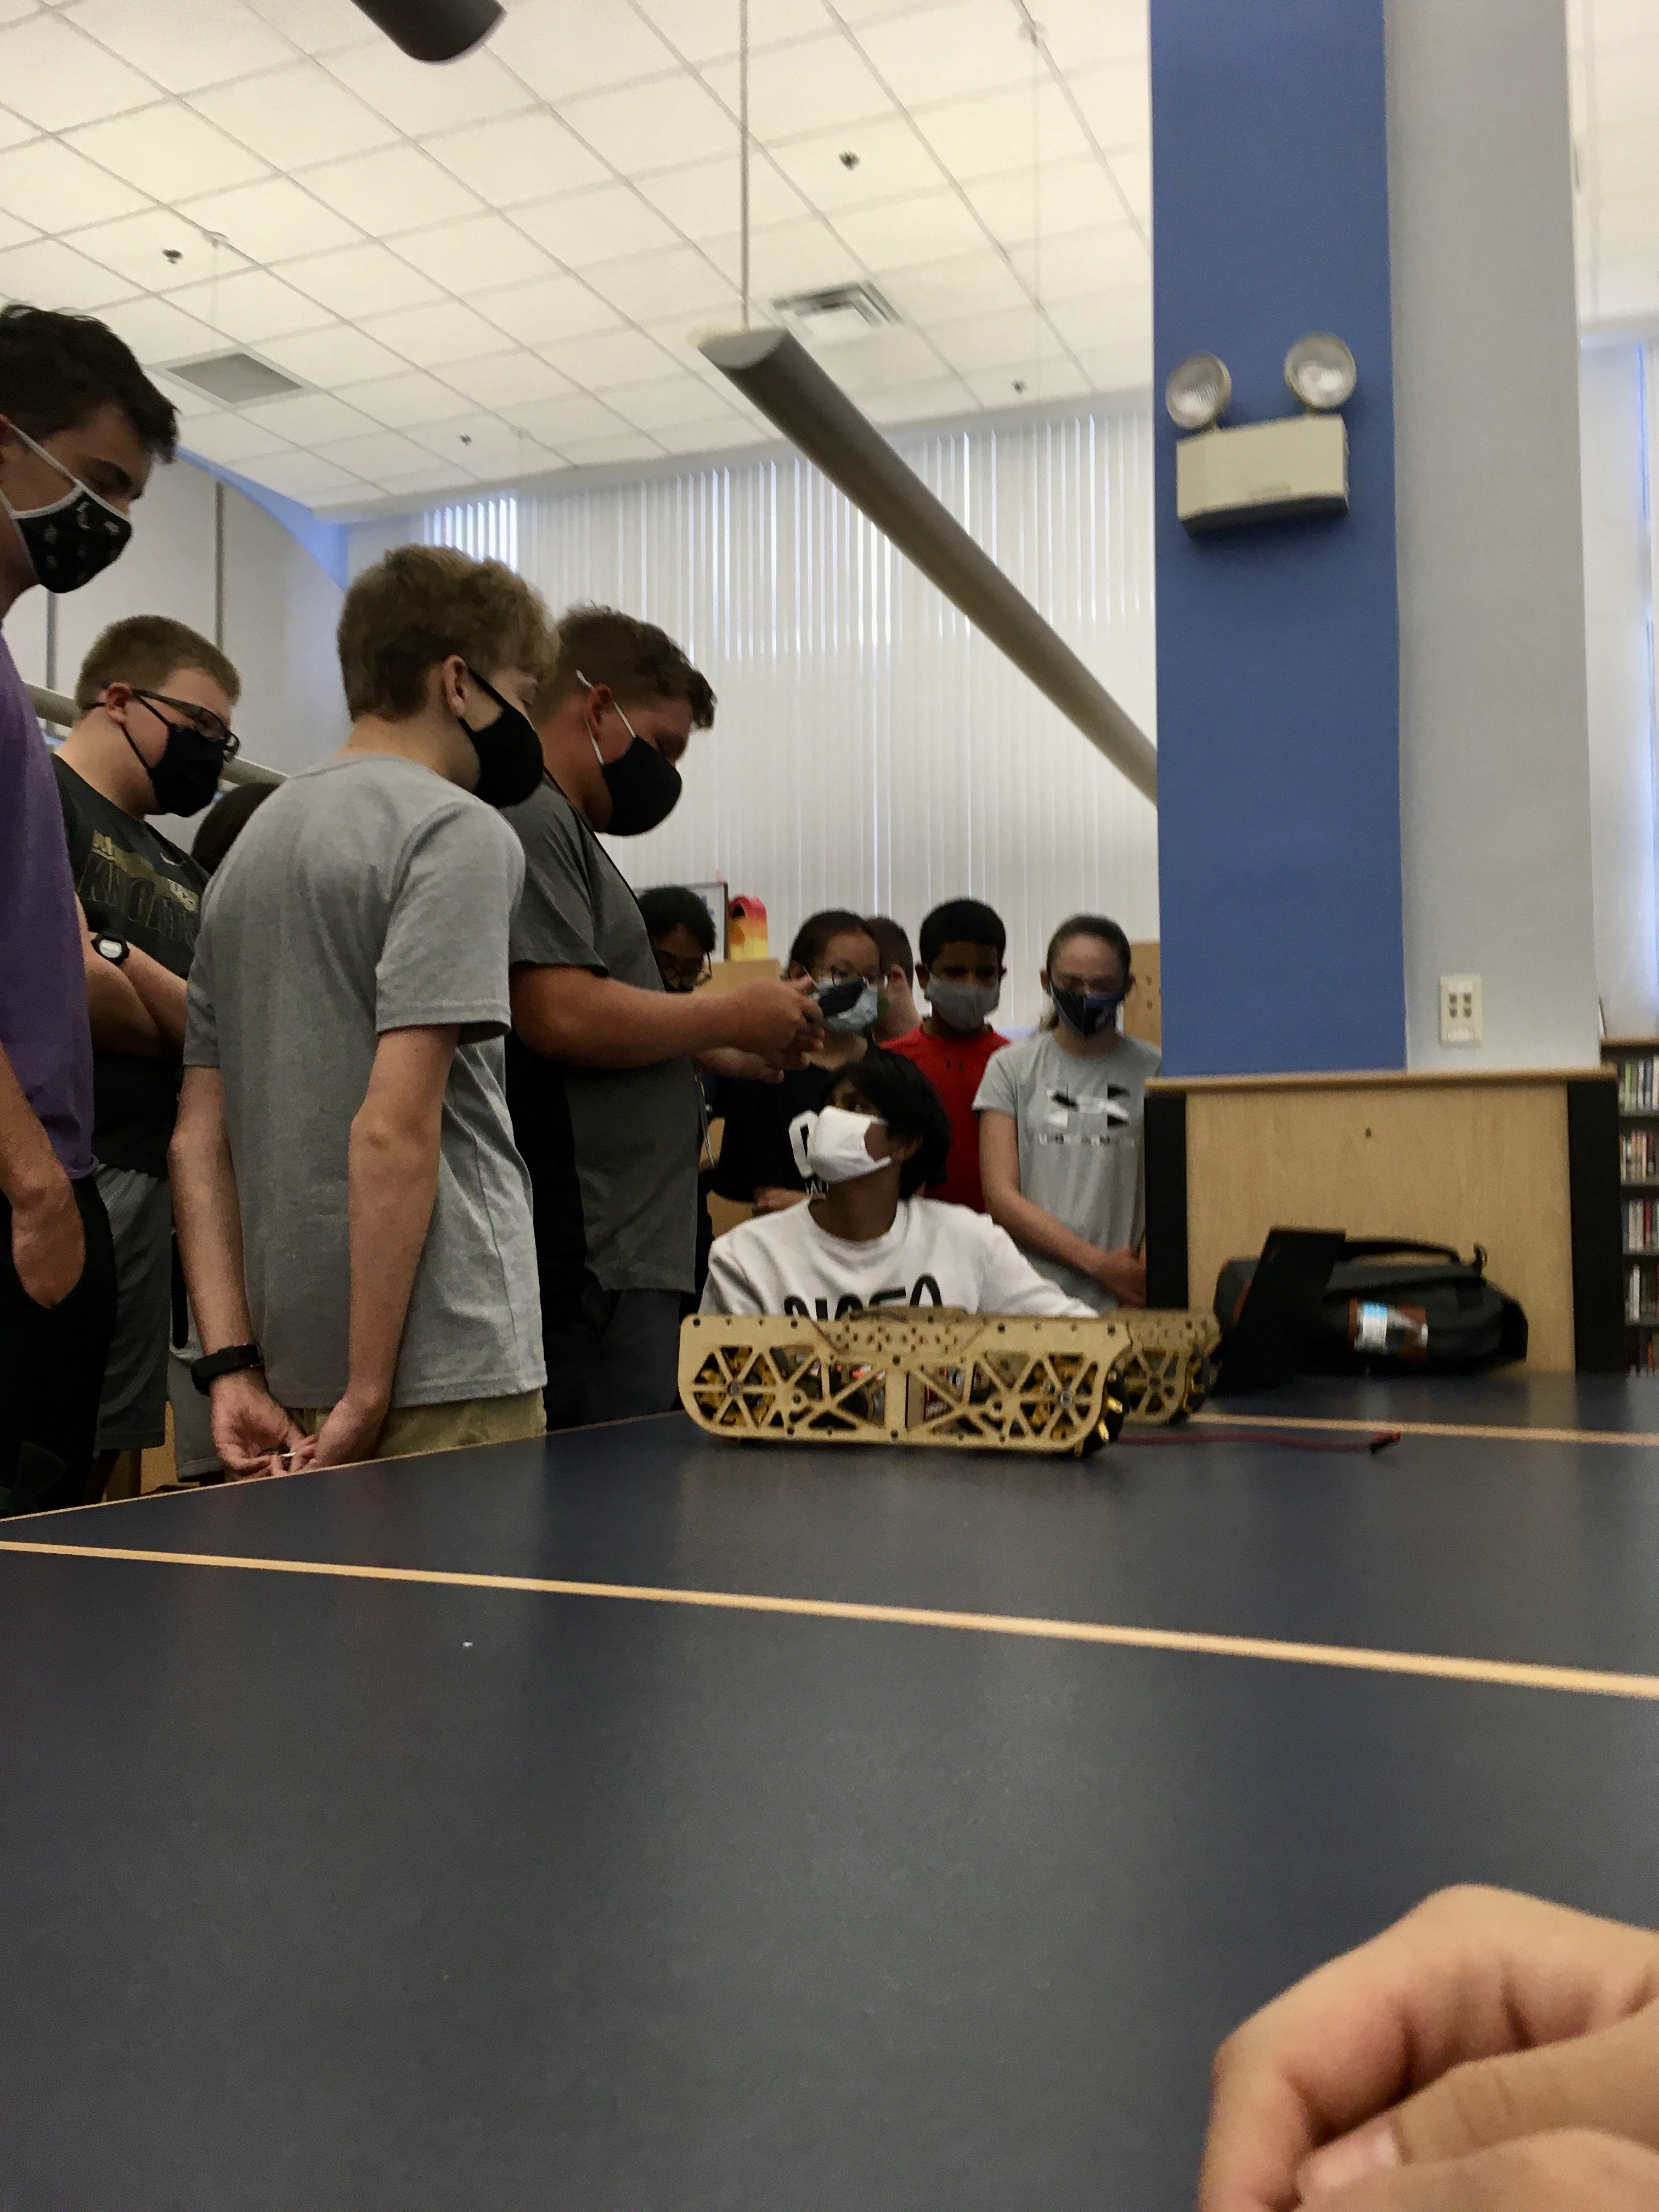
\includegraphics[width=0.9\textwidth, angle=0]{Meetings/August/08-18-21/08-18-21 1.JPG}
  \caption{Ritam helping show younger members the fundamentals of CAD.}
  \label{fig:081821_1}
\end{minipage}
\begin{minipage}[b]{.48\textwidth}
  \centering
  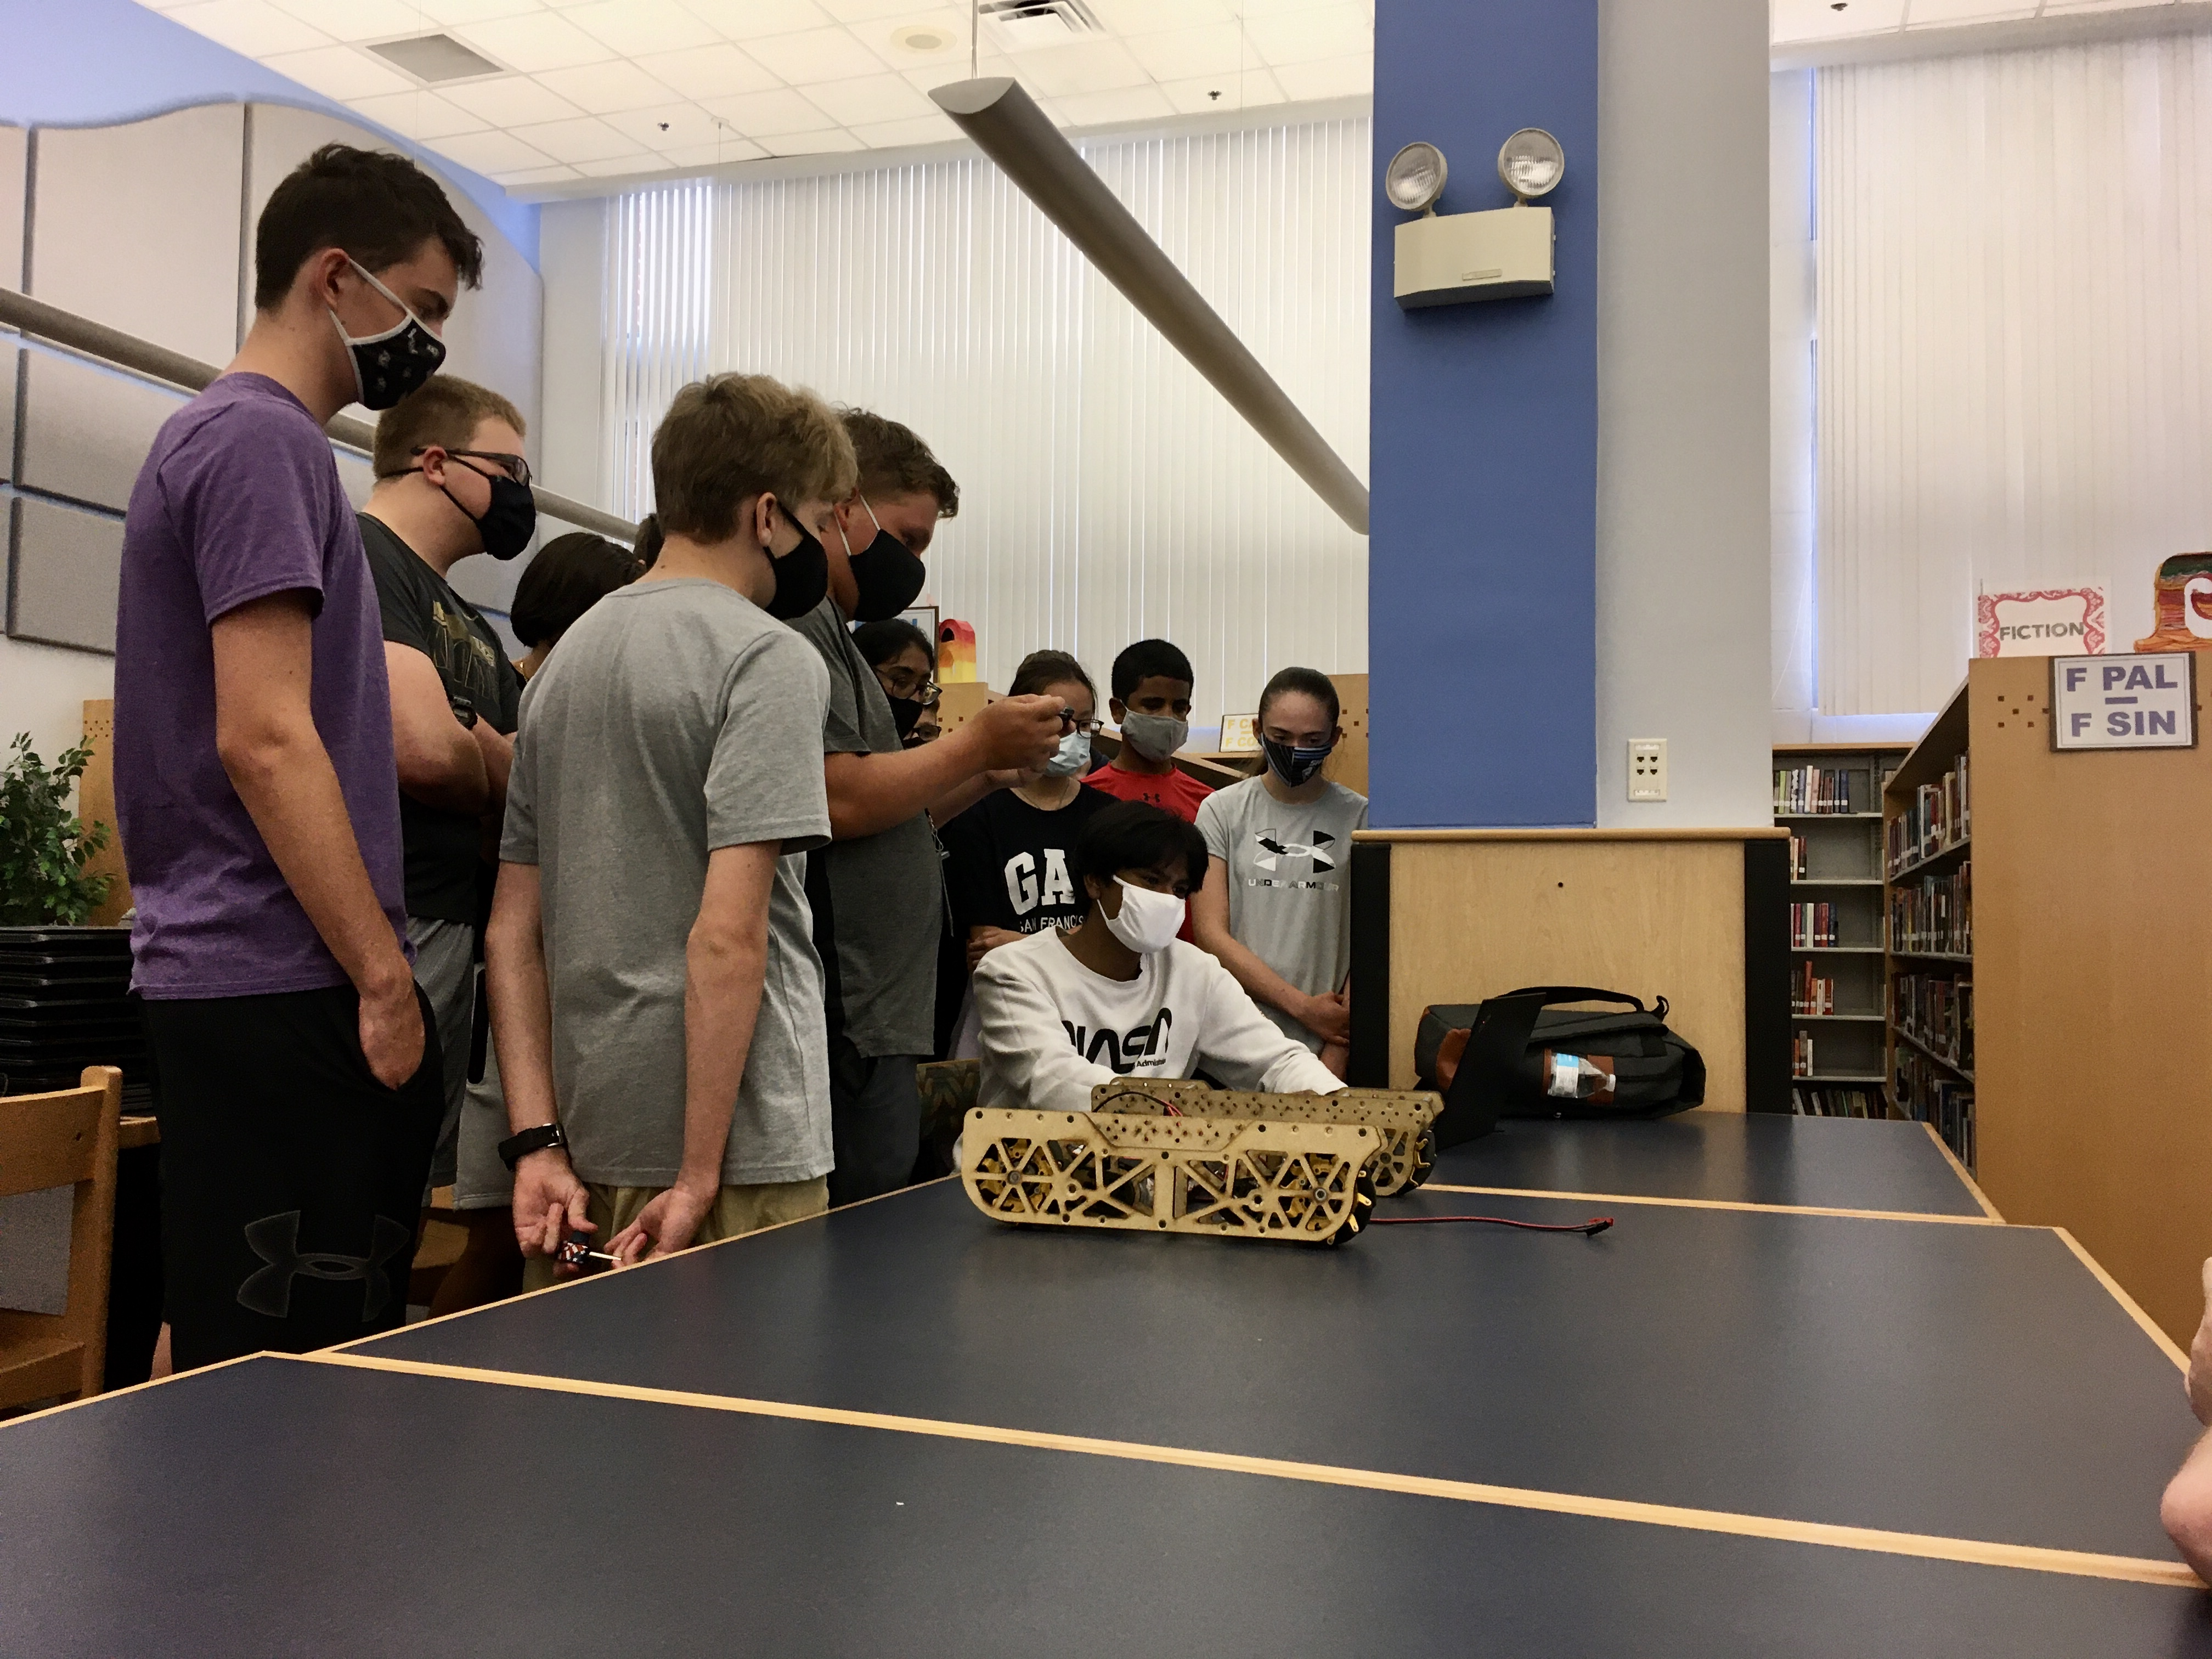
\includegraphics[width=0.9\textwidth, angle=0]{Meetings/August/08-18-21/08-18-21 2.JPG}
  \caption{More Ritam helping show younger members the fundamentals of CAD.}
  \label{fig:081821_2}
\end{minipage}
\end{figure}

\hhscommittee{Hardware}
\noindent\hfil\rule{\textwidth}{.4pt}\hfil
\subsubsection*{Goals}
\begin{itemize}
    \item Finish cutting rev hub mount
	\item Put together rev hub mounts
	\item Cut churros
  

\end{itemize} 

\noindent\hfil\rule{\textwidth}{.4pt}\hfil

\subsubsection*{Accomplishments}
Because our main goal for this meeting was to put together the rev hub mount, we started by continuing to cut out all of the pieces of the assembly. We set up the glowforge laser cutter once again and put our ¼ inch wood in the machine and cut the remaining parts. Once the pieces had finished cutting, we had all 6 wooden parts and were ready to start building.(Figure \ref{fig:081821_1})
Thanks to our use of box joints and t-slot joints in cad, we were able to put the whole assembly together relatively easily and quickly. (Figure \ref{fig:081821_2}) one thing we noticed was that not all of the box joints held firmly, which was somewhat troubling where we had neglected to add t-slot joints. In the future we need to be less conservative with the t-slot joints. Other than that, the assembly went together smoothly. 
Our next step was to cut down metal churros, metal poles that will connect the two halves of our drivetrains. The churros were 17 inches to start off with and we needed them to be 16 inches. We marked where we needed to cut them and clamped them into a grinder (Figure \ref{fig:081821_3}). After cutting the churros, we smoothed the ends out on the belt sander because the grinder left them a bit rough. Unfortunately, the churros were not threaded all the way through, so we were unable to attach them to the rest of the robot. This means that for tele-op testing we will have to find another way to attach the sides. Luckily, we were prepared for this scenario because of the tetrix holes that we added onto the inner drive plates that will allow us to make quick modifications like the one that we need. Despite not using the churros until we can thread them, we still put them through the battery holder to ensure that the holes were the right size, finding that the churros fit as expected.(Figure \ref{fig:081821_4}). 

\begin{figure}[ht]
\centering
\begin{minipage}[b]{.48\textwidth}
  \centering
  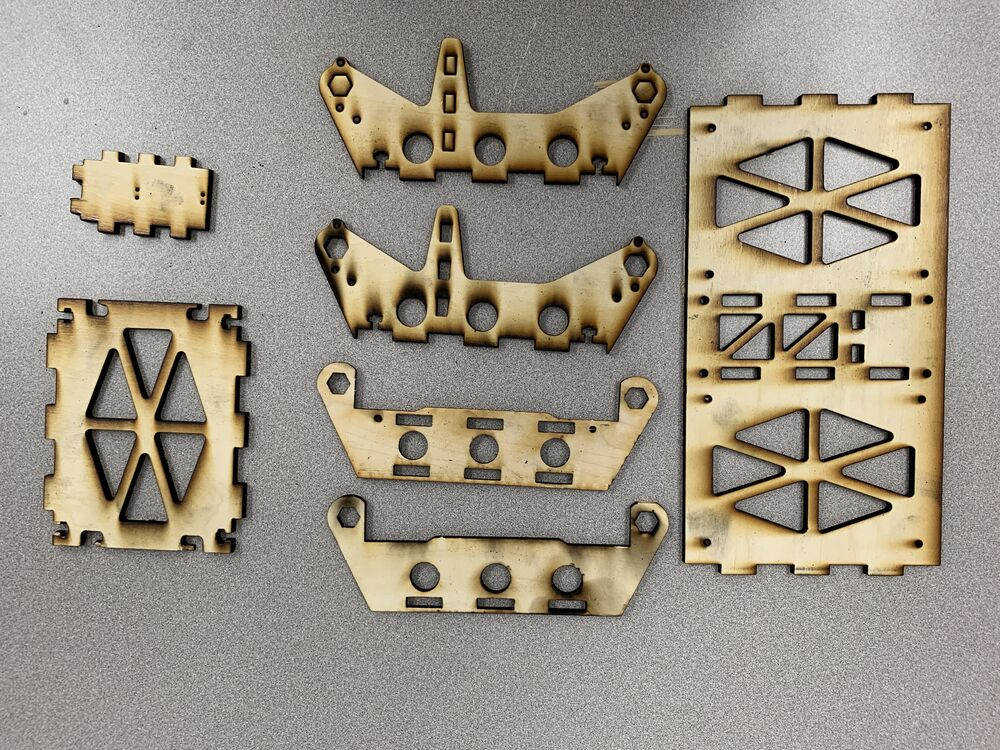
\includegraphics[width=0.95\textwidth]{Meetings/August/08-18-21/8-18-21_hardware_img1 - Nathan Forrer.JPG}
  \caption{Plates cut for our Rev Hub mounts.}
  \label{fig:081821_1}
\end{minipage}%
\hfill%
\begin{minipage}[b]{.48\textwidth}
  \centering
  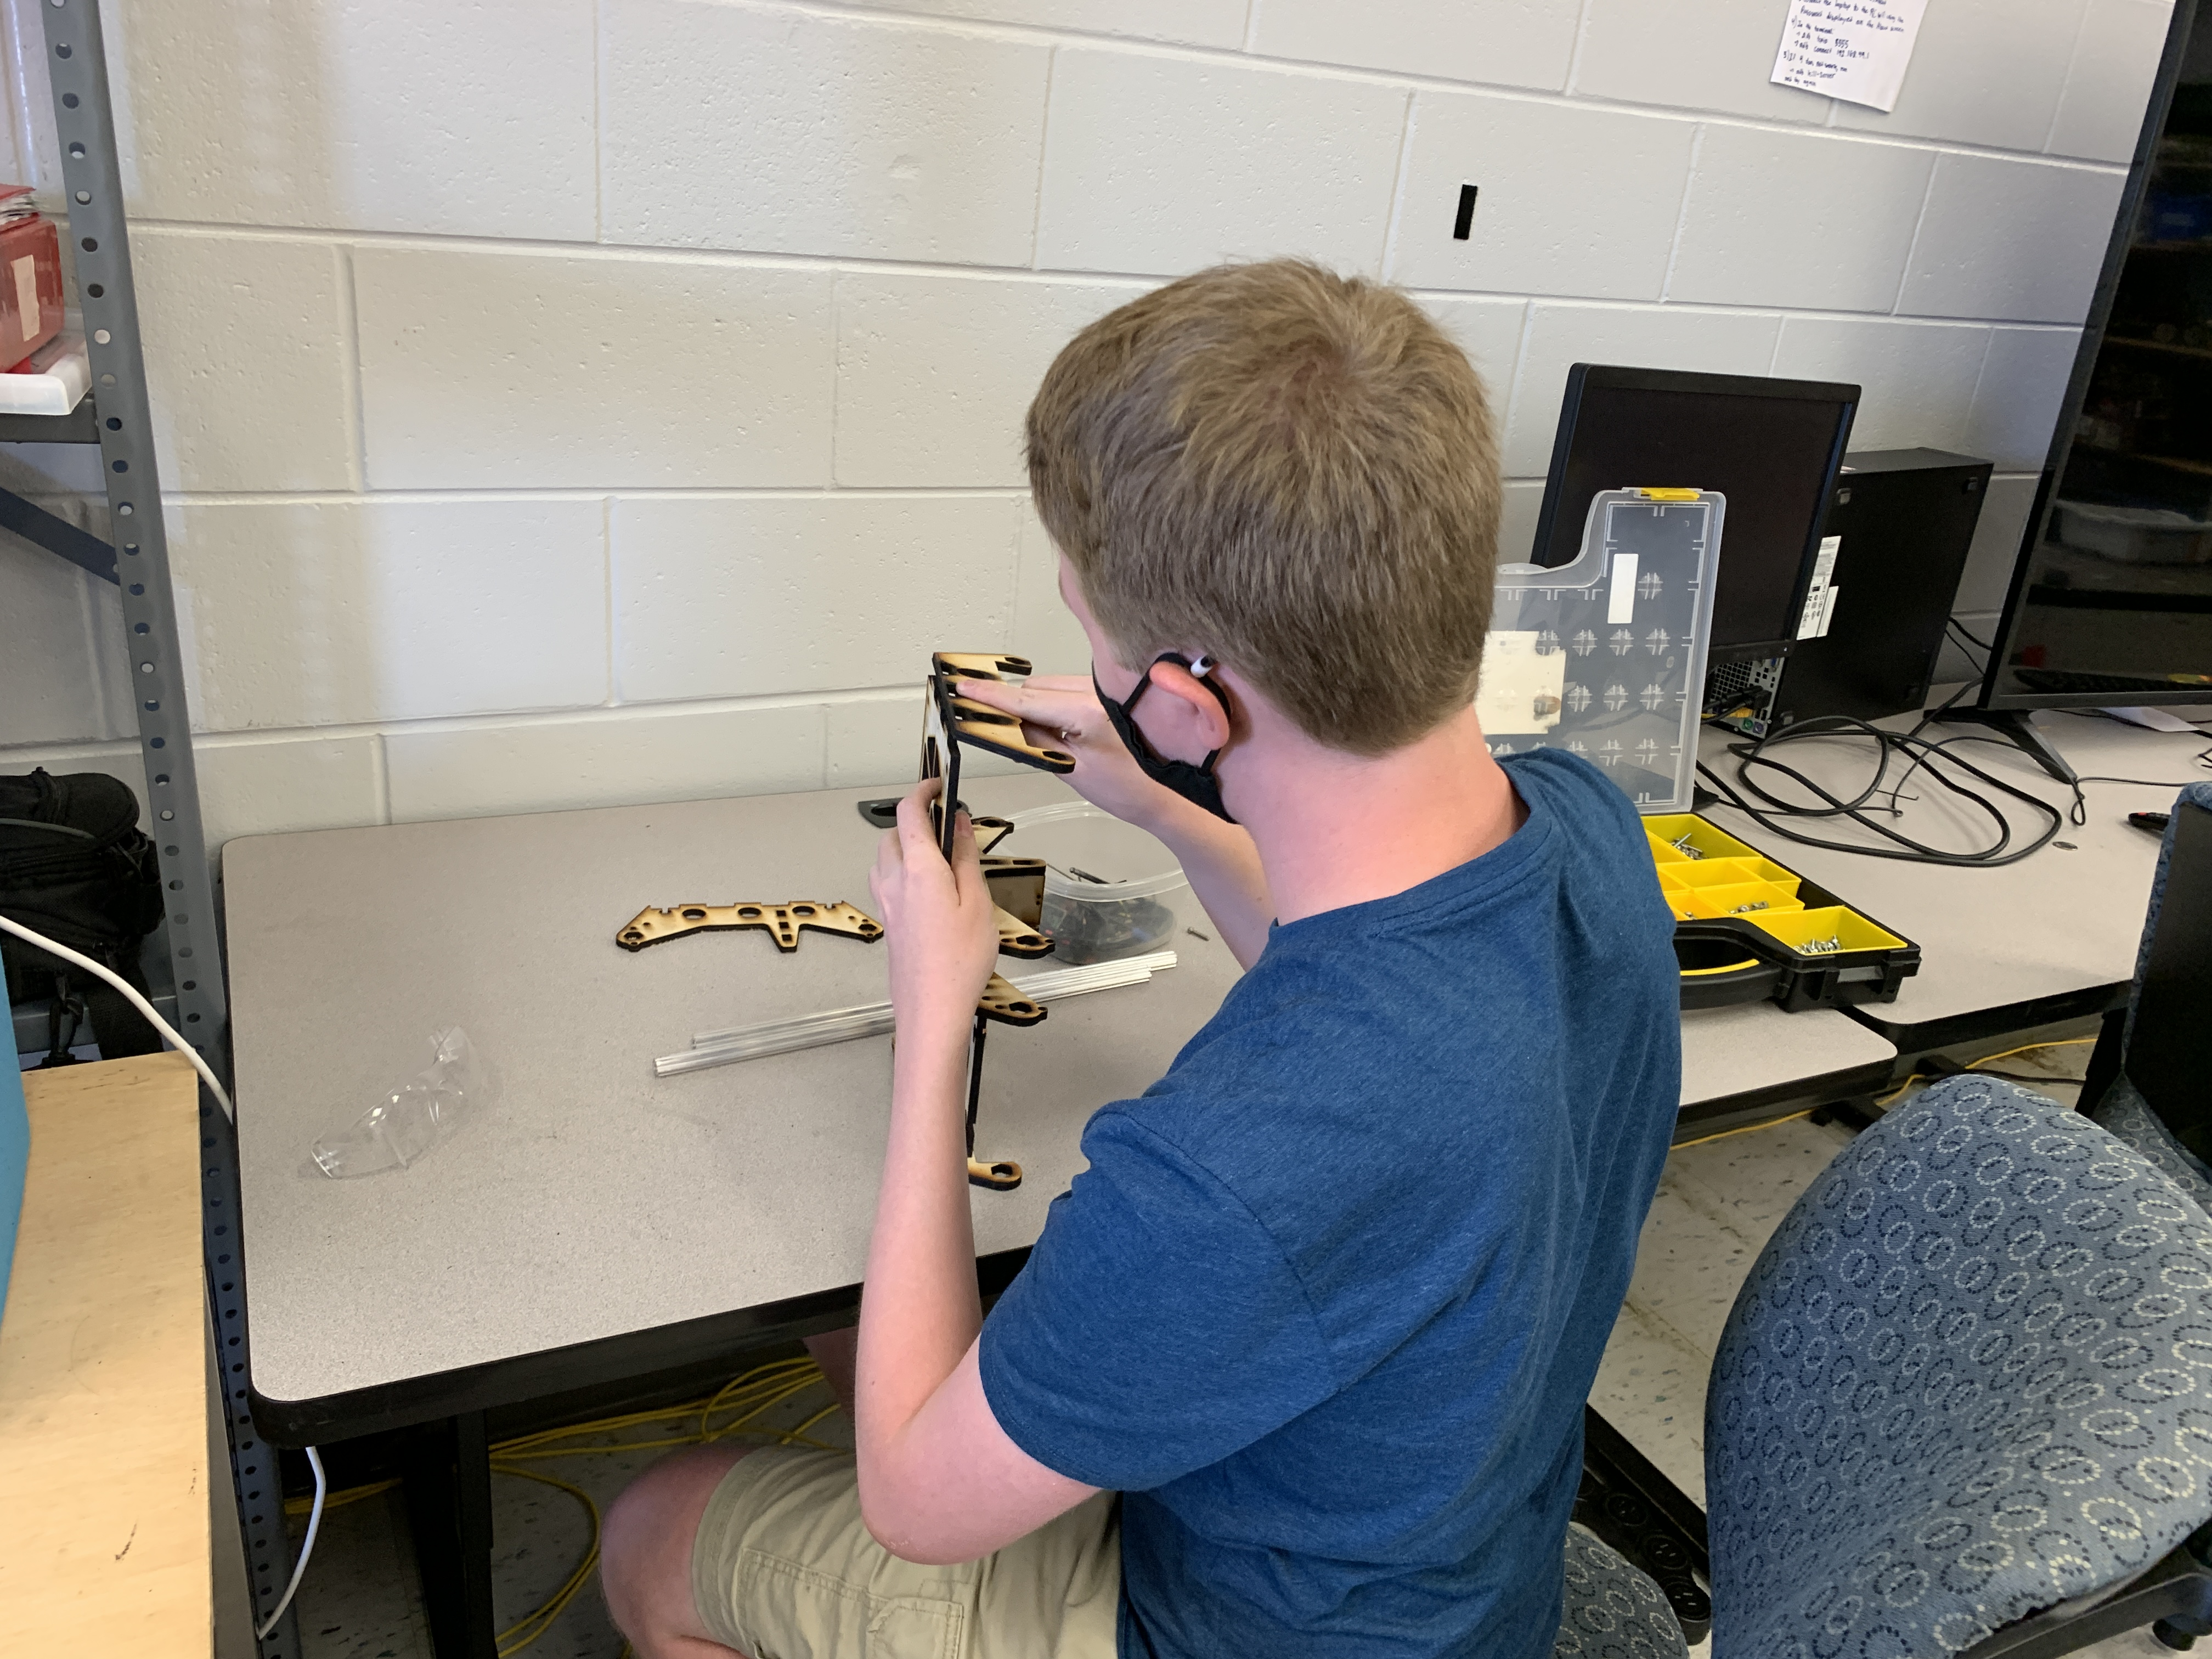
\includegraphics[width=0.95\textwidth]{Meetings/August/08-18-21/8-18-21_hardware_img2 - Nathan Forrer.JPG}
  \caption{Nathan assembling our pieces.}
  \label{fig:081821_2}
\end{minipage}
\end{figure}

\begin{figure}[ht]
\centering
\begin{minipage}[b]{.48\textwidth}
  \centering
  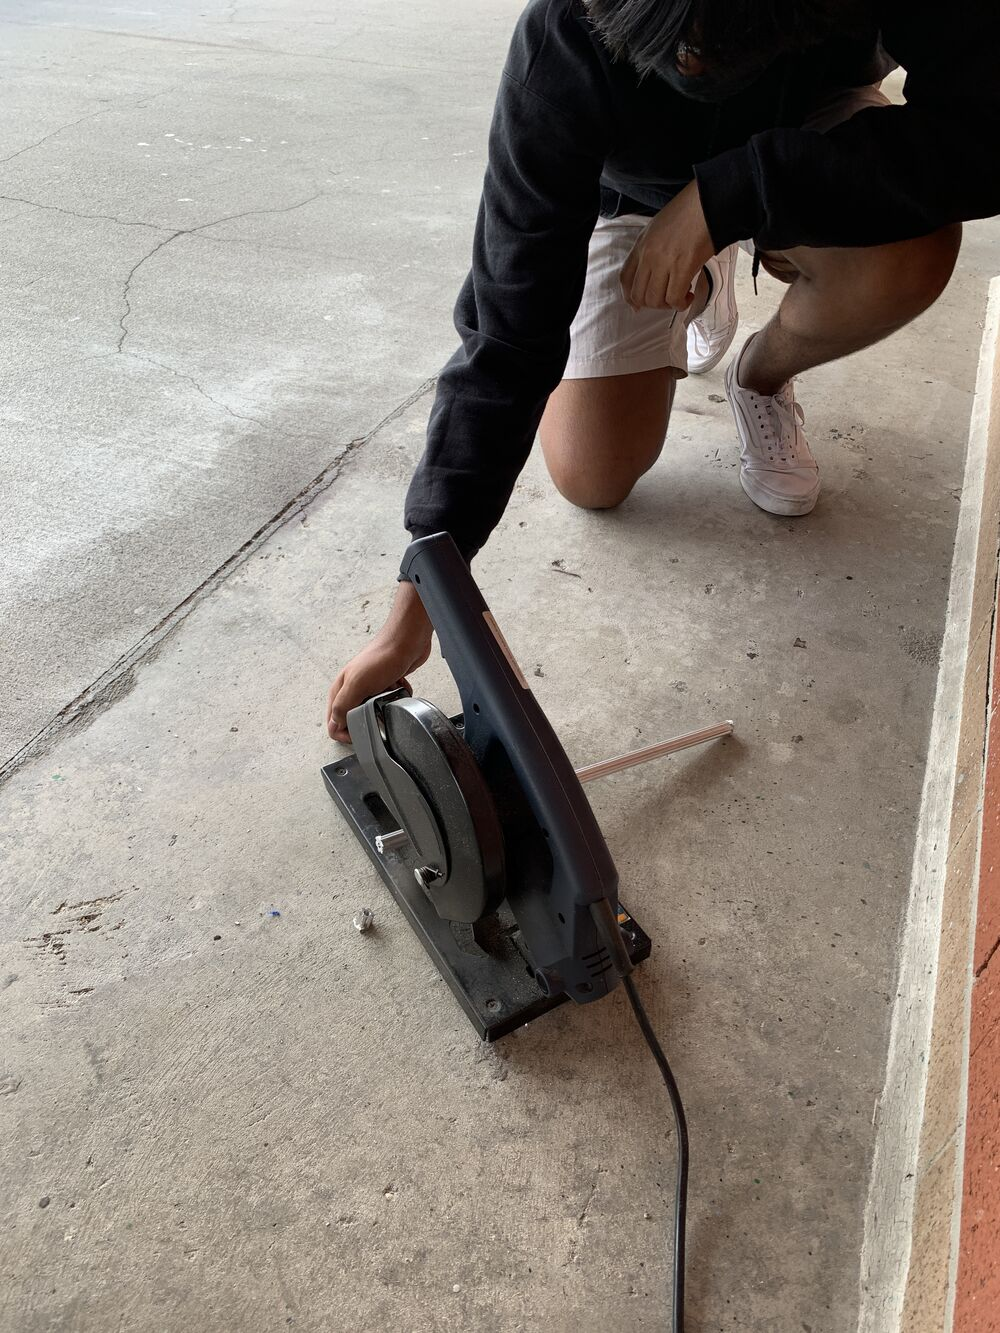
\includegraphics[width=0.95\textwidth]{Meetings/August/08-18-21/8-18-21_hardware_img3 - Nathan Forrer.JPG}
  \caption{Cutting churros to smaller lengths to hold our drive plates together.}
  \label{fig:081821_3}
\end{minipage}%
\hfill%
\begin{minipage}[b]{.48\textwidth}
  \centering
  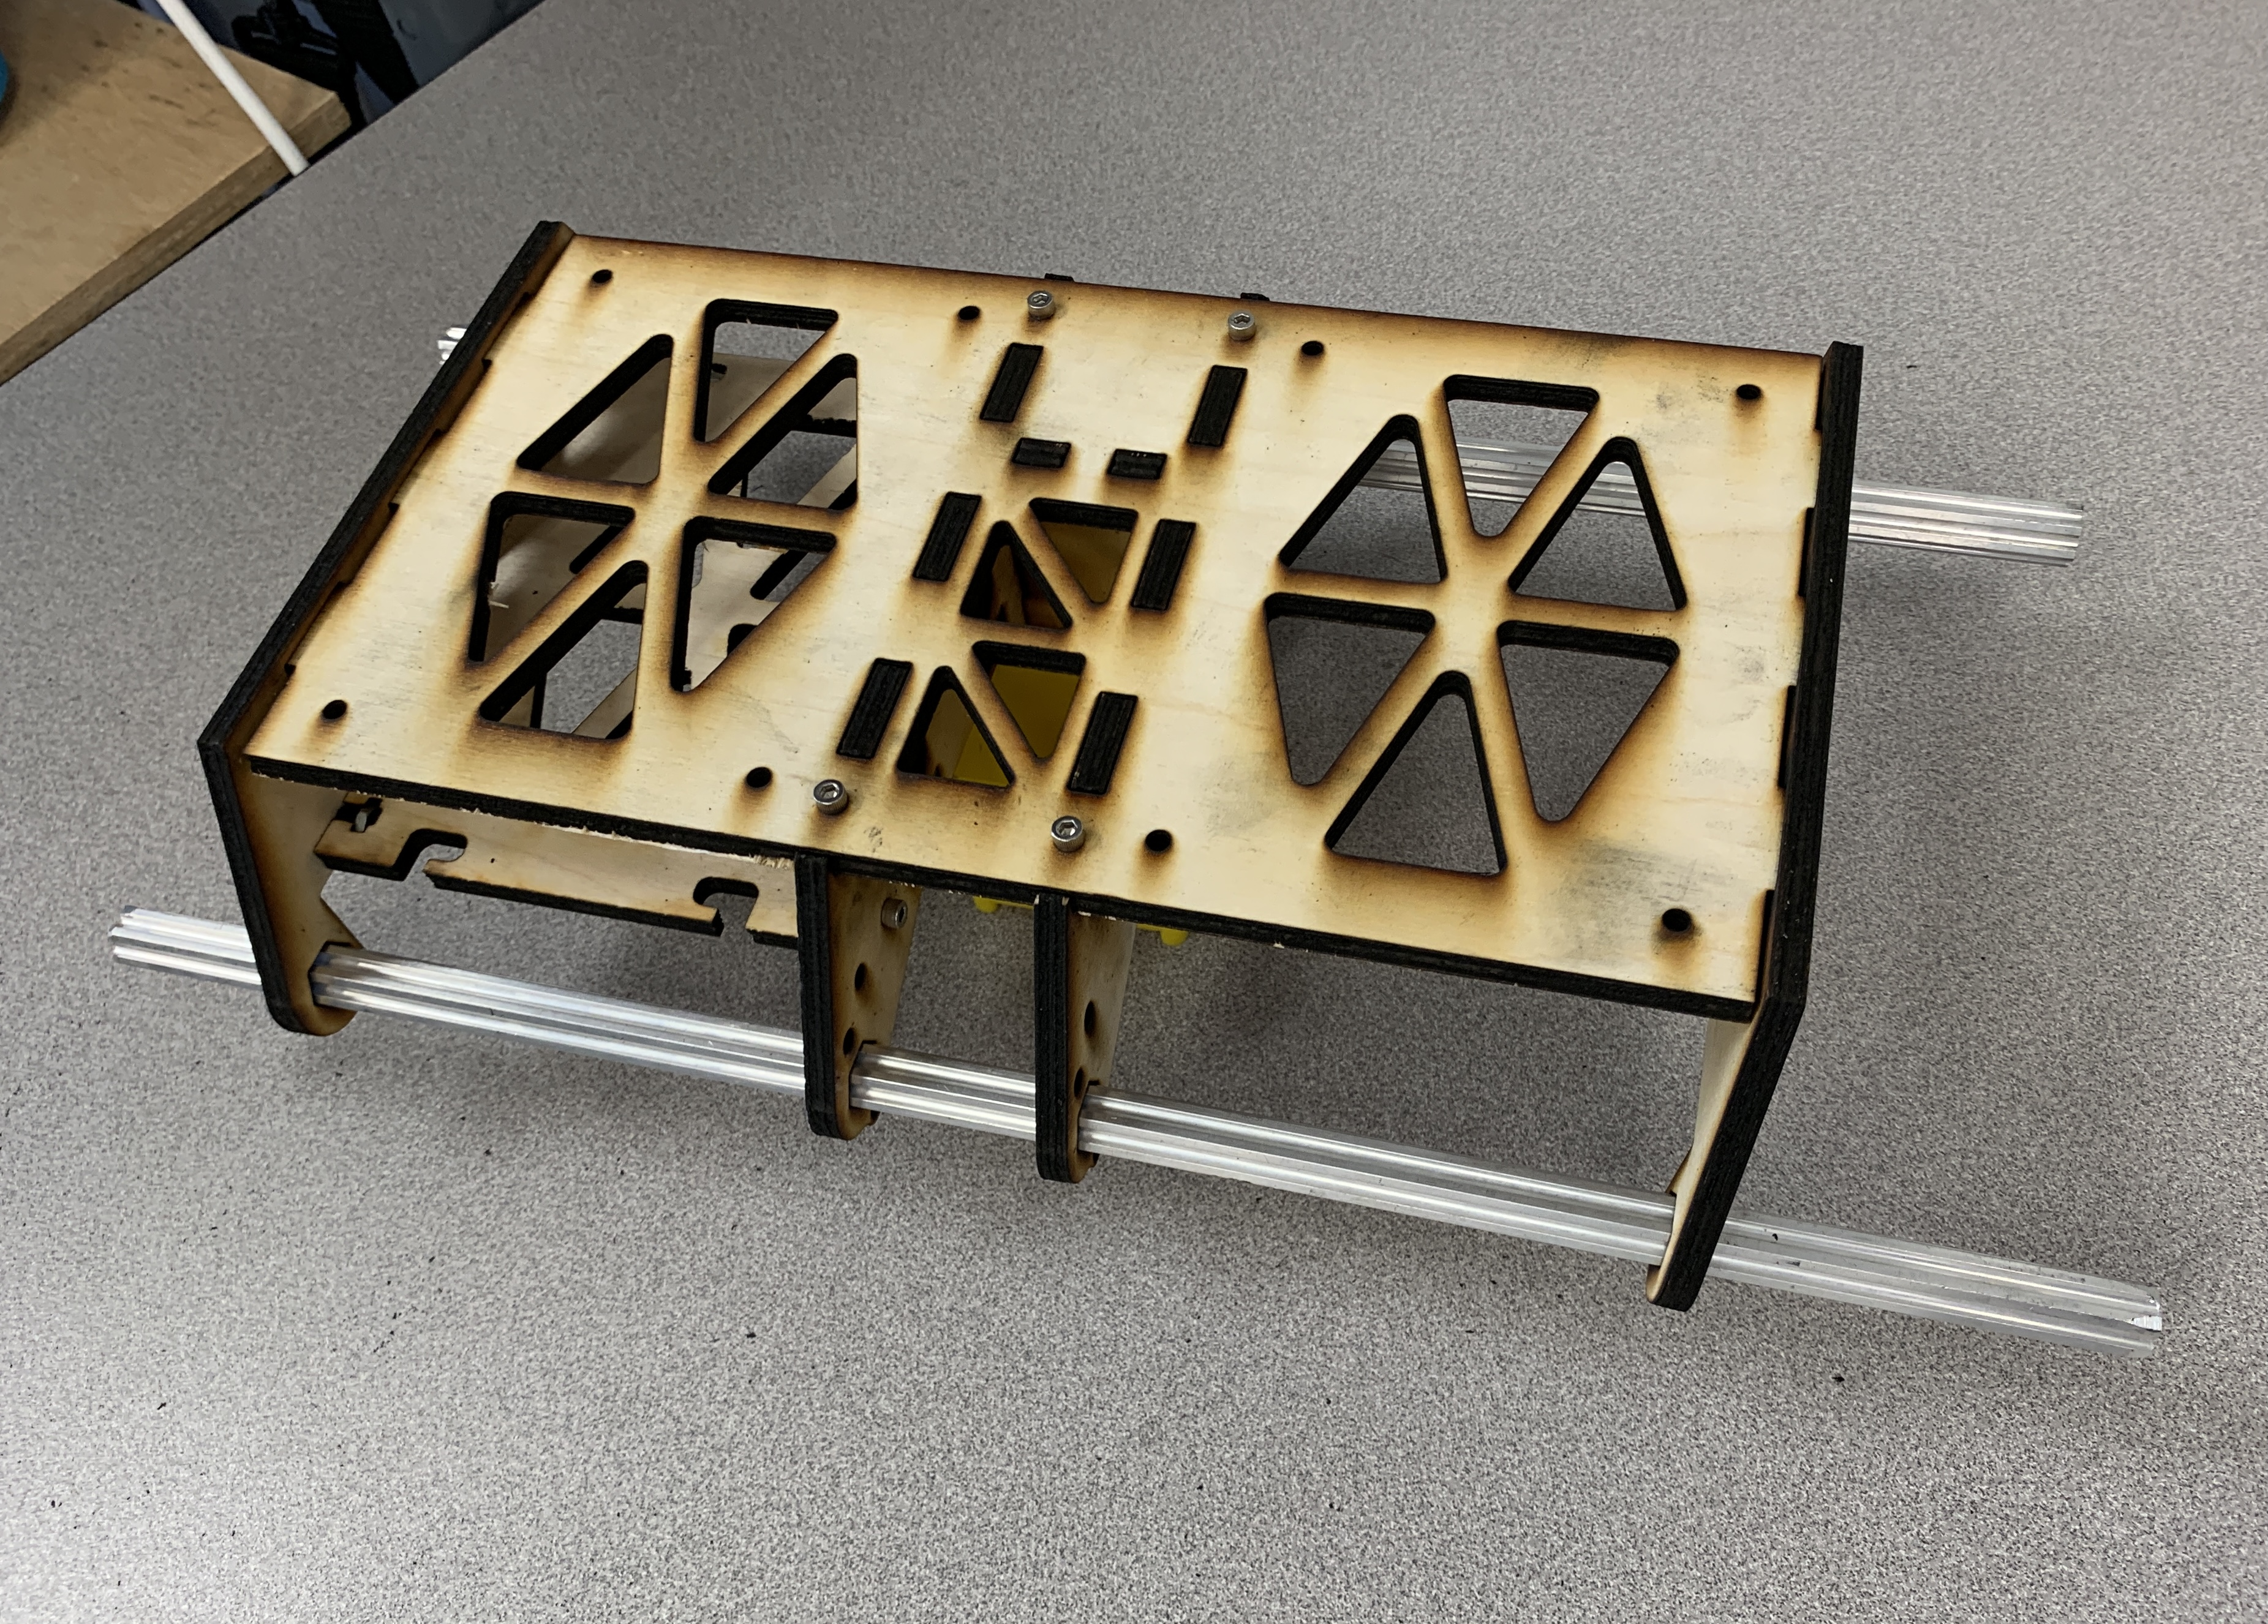
\includegraphics[width=0.95\textwidth]{Meetings/August/08-18-21/8-18-21_hardware_img4 - Nathan Forrer.JPG}
  \caption{Our assembled Rev Hub mount, complete with churros, ready to attach to our soon-to-be completed drivetrain.}
  \label{fig:081821_4}
\end{minipage}
\end{figure}

\whatsnext{
\begin{itemize}
    \item Design intake prototypes
    \item Connect drivetrain
    \item Thread churros
\end{itemize} 
}